\documentclass{standalone}
\usepackage{mathpazo}
\usepackage{tikz}
\usetikzlibrary{calc}
\usetikzlibrary{arrows}

\usepackage[american voltages, american inductors, american currents, european resistors]{circuitikz}

\begin{document}
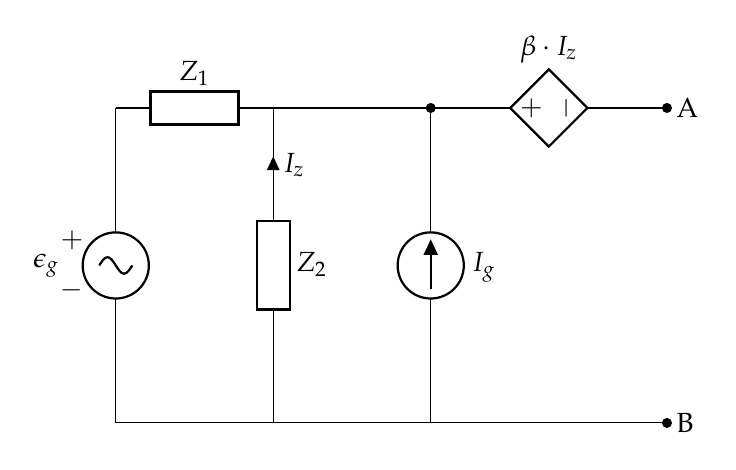
\begin{tikzpicture}
  \coordinate (A) at (0,0);
  \coordinate (B) at ($(A) + (2,0)$);
  \coordinate (C) at ($(B) + (2,0)$);
  \coordinate (D) at ($(C) + (3,0)$);
  \coordinate (E) at ($(A) + (0,-4)$);
  \coordinate (F) at ($(E) + (2,0)$);
  \coordinate (G) at ($(F) + (2,0)$);
  \coordinate (H) at ($(G) + (3,0)$);
  \draw
  (A) to [R, l = $Z_1$] (B)
  to [short, -*] (C)
  (E) to [short, -*] (H) node[right] {B}
  (A) to [sV, v_=$\epsilon_g$] (E)
  (G) to [isource, l_= $I_g$] (C)
  (B) to [R, l = $Z_2$, i<= $I_z$] (F)
  (C) to [cV, l = $\beta \cdot I_z$, -*] (D) node[right] {A};
\end{tikzpicture}
\end{document}